
\documentclass[colorinlistoftodos]{article} % For LaTeX2e
\usepackage{iclr2020_conference,times}

% Optional math commands from https://github.com/goodfeli/dlbook_notation.
\input{math_commands.tex}

\usepackage{hyperref}
\usepackage{url}
\usepackage[algo2e,ruled,linesnumbered,lined]{algorithm2e}

\usepackage[english]{babel}
\usepackage[utf8]{inputenc}
\usepackage{algorithm}
% \usepackage{arevmath}     % For math symbols
\usepackage[noend]{algpseudocode}
\usepackage{graphicx}


\newcommand\mynotesEB[1]{\textcolor{red}{#1}}
\newcommand\mynotesLC[1]{\textcolor{blue}{#1}}
\setlength{\marginparwidth}{3cm}
\usepackage{amssymb,todonotes}
\usepackage{wrapfig}



\title{Online Learned Continual Compression with Stacked Quantization Modules}
%via Stacked Quantization Modules}

% Authors must not appear in the submitted version. They should be hidden
% as long as the \iclrfinalcopy macro remains commented out below.
% Non-anonymous submissions will be rejected without review.

\author{Lucas Caccia$^{1}$, Eugene Belilovsky$^{2}$, Massimo Caccia$^{2}$ \& Joelle Pineau$^{1,3}$
\thanks{$^1$ MILA, McGill University, $^2$ MILA University of Montreal, $^3$ Facebook AI Research (FAIR). \texttt{ lucas.page-caccia@mail.mcgill.ca}}}

% The \author macro works with any number of authors. There are two commands
% used to separate the names and addresses of multiple authors: \And and \AND.
%
% Using \And between authors leaves it to \LaTeX{} to determine where to break
% the lines. Using \AND forces a linebreak at that point. So, if \LaTeX{}
% puts 3 of 4 authors names on the first line, and the last on the second
% line, try using \AND instead of \And before the third author name.

\newcommand{\fix}{\marginpar{FIX}}
\newcommand{\new}{\marginpar{NEW}}

% \iclrfinalcopy % Uncomment for camera-ready version, but NOT for submission.
\begin{document}


\maketitle

\begin{abstract}
% Online continual learning studies models' and agents' ability to learn when samples are observed only once and tasks arrive sequentially. Some retention of previous tasks information is required for the learner to remember how they are performed, while learning new ones. This inevitably leads us into scalability issues due to the ever-increasing memory cost. We thus introduce and study the problem of Online Continual Compression.

We introduce and study the problem of Online Continual Compression, where one attempts to learn to compress and store a representative dataset from a non i.i.d data stream, while only observing each sample once. This problem is highly relevant for downstream online continual learning tasks, as well as standard learning methods under resource constrained data collection. To address this we propose a new architecture which Stacks Quantization Modules (SQM), consisting of a series of discrete autoencoders, each equipped with their own memory. Every added module is trained to reconstruct the latent space of the previous module using fewer bits, allowing the learned representation to become more compact as training progresses. This modularity has several advantages: 1) moderate compressions are quickly available early in training, which is crucial for remembering the early tasks, 2) as more data needs to be stored, earlier data becomes more compressed, freeing memory, 3) unlike previous methods, our approach \textit{does not require pretraining}, even on challenging datasets. We show several potential applications of this method. We first replace the episodic memory used in Experience Replay with SQM, leading to significant gains on standard continual learning benchmarks using a fixed memory budget. We then apply our method to online compression of larger images like those from Imagenet, and show that it is also effective with other modalities, such as LiDAR data.

\end{abstract}

% \listoftodos
% ---------------------------------------------------------
%                       INTRODUCTION
% ---------------------------------------------------------

\section{Introduction}

%\subsection{Motivation for Online Continual Compression}
%Intro paragraph about learned compression
Interest in machine learning in recent years have been fueled by the plethora of data being generated on a regular basis. Effectively storing and using this data is critical for many applications, especially those involving continual learning. In general, compression techniques can greatly improve data storage capacity, and, if done well, reduce the memory and compute usage in downstream machine learning tasks \citep{JPEG,Oyallon_2018_ECCV}. Thus, learned compression has become a topic of great interest \citep{theis2017lossy,balle2016end,johnston2018improved}. Yet its application in reducing the size of datasets bound for machine learning applications has been limited.

%Continual online compression has some natural use cases  
This work focuses on the following familiar setting: new training data arrives continuously for a learning algorithm to exploit, however this data might not be iid, and furthermore there is insufficient storage capacity to preserve all the data uncompressed. We may want to train classifiers, reinforcement learning policies, or other models continuously from this data, or use samples randomly drawn from it at a later point for a downstream task. For example, an autonomous vehicle (with bounded memory) collects large amounts of high-dimensional training data (video, 3D lidar) in a non-stationary environment (e.g. changing traffic patterns), and overtime applies an ML algorithm to improve its behavior using this data. This data might be transferred at a later point for use in downstream supervised learning. Current standard learned compression algorithms, e.g. \cite{torfason2018towards}, are not well designed to deal with this case,  \mynotesLC{as their convergence speed is too slow to be usable in an online setting.}

In the field of continual/lifelong learning \citep{thrun1995lifelong}, which has for now largely focused on classification, approaches based on storing memories for later use have emerged as some of the most effective in online settings \citep{lopez2017gradient,aljundi2018Online,chaudhry2018efficient,chaudhry2019continual,aljundi2019online}. These memories can be stored as is, or via a generative model \citep{shin2017continual}. Then, they can either be used for rehearsal \citep{chaudhry2019continual,aljundi2019online} or for constrained optimization \cite{lopez2017gradient,chaudhry2018efficient,aljundi2018Online}.
Indeed many continual learning applications would be nearly solved with replay approaches if one could afford to store all samples. These approaches are however inherently limited by the amount of data that can be stored\footnote{This is typically not feasible for on-device machine learning. And while many ML services currently run on the cloud, the move towards increasingly higher data privacy standards is likely to push many ML algorithms to run locally on device.}.

Learning a generative model to compress the previous data stream thus seems like an appealing idea. However, learning generative models, particularly in the online (possibly non-stationary) setting, continues to be challenging, and can greatly increase the complexity of the continual learning task. Furthermore, such models are susceptible to catastrophic forgetting \cite{aljundi2019online}. 
An alternate approach is to simply learn a compressed representation of the data; this is typically faster and more stable than learning to generate the whole data distribution. While the learned compression may itself exhibit forgetting and representation drift, causing challenges for continual and online cases, a learned compression method that can learn continuously and online would allow the storing of far larger amount of samples for replay.


In this work we investigate the use of quantized autoencoders, specifically the VQ-VAE framework \cite{van2017neural}, observing that these can learn continuously and online with minimal forgetting, particularly when augmented with their own internal rehearsal mechanisms. We propose a multi-level stacked model that allows the compressor to adaptively store samples at different compression scales, based on the amount of data, storage capacity, and effectiveness of the model in compressing samples. Furthermore, the learned compressed representation allows multiple continual learning models to be trained from the same data.

%\todo[color=green]{add motivation related to huge amount of data to compress problem}
The main contributions in this work are as follows: (a) we introduce and highlight the importance of the online continual learned compression problem; (b) we demonstrate how Multi-level VQ-VAE, combined with internal replay, can effectively learn compressed representations of online data, (c) we show online learned compression can yield state-of-the-art performance in standard online continual image classification benchmarks.

%\begin{enumerate}
	%\item Learned Compression (in general)
	%\begin{enumerate}
	%	\item  Amount of data being generated on a regular basis is huge (cite article Mass was referencing). 
	%	\item Reduce storage burden, Make the most of your storage capacity (especially for high-performance / low memory hardware like GPU)
	%\end{enumerate}

	%\item Online Compression
	%			\begin{enumerate}
	%				\item There might not always be pretrained models available for all data types (think of LiDAR for example). The need sample efficient convergence / performance can be crucial, especially for applications where collecting data is expensive (more in the robotics section)
	%			
	%			\end{enumerate}						

	
%	\item Robotics Perspective 
%		\begin{enumerate}
%			\item  Deploying robots for high-dimensional data collection in the wild. 
		
%			\begin{enumerate}
%				\item Scenario A: Robot is collecting data without access to internet, and with limited storage capacity. There is an overhead cost for it to come back to a docking station and transmit its data. E.g a rover on the moon. 
%				\item Scenario B: Robot must transmit data over bandwidth. Less bits transmitted $\rightarrow$ Cost of transmission is reduces		
%			\end{enumerate}	
			
%			\item Expensive to operate robots (I would assume Le Bras Canadien in space is one of them). If you are going to train an AI to perform some complex manipulation task, you will want to train it with a few samples as possible. (This is more to motivate the \textit{online} part.	 
		
%		\end{enumerate}				
			
		%\item Continual Learning
		%	\begin{enumerate}
			%	\item Storing data (and compressed versions of it) is much more robust to forgetting (than regular approaches); \textbf{the data holds all the information you need to train a model}. The problem is that memory quickly becomes the main hurdle to overcome. By compressing the data you can alleviate this obstacle. 
			%	\item Small Note: I would like to stress the point above, that most online CL application would be solved with memory-based approaches if you could afford to store all samples.
			%	\item SOTA methods for CL are largely rehearsal based.  Same argument as below: storing compressed representations not only allows you to store more, but makes rehearsal more efficient
		%	\end{enumerate}
			
				
	%	\item Deep Learning Perspective
	%		\begin{enumerate}
	%			\item Memory NNs / Nonparametric Approaches
	%			\begin{enumerate}
	%				\item GPU memory is small and limited. A major bottleneck in training models is the RAM to GPU transfer. If you are dealing with compressed representations the transfer time per example is smaller, hence makes training faster. 
	%				\item This would be especially true for networks that leverage an external memory during training / inference (hence the title). 
	%			\end{enumerate}		

	%		\end{enumerate}
 
%\end{enumerate}

%\todo[color=green]{finish introduction}


% ---------------------------------------------------------
%                       RELATED WORK
% ---------------------------------------------------------
\section{Related Work}

\paragraph{Learned compression} has been recently studied for the specific case of image compression. Work by \citet{theis2017lossy,balle2016end,johnston2018improved} have shown learned compressions can outperform standard compression algorithms like JPEG. Some of these methods however are challenging to train, thus in our work we focus on the VQ-VAE approach \cite{van2017neural,razavi2019generating} which allows us to address online continual learning settings and permit a multi-level storage. 

%SOMETHING THAT INTRODUCES THE SUBSECTIONS
%\subsection{Continual Learning}
\paragraph{Continual Learning} research currently focuses on overcoming catastrophic forgetting (CF) in the supervised learning setting, with some limited work in the generative modeling and reinforcement learning settings. Most continual learning methods can be grouped into three major families. 

Some algorithms dynamically change the model’s architecture to incorporate learning from each task separately. Popular methods are \citet{rusu2016progressive}, \citet{li2018learning} and  \citet{fernando2017pathnet}. Although these methods can perform well in practice, their introduction of task-specific weights requires growing compute and memory costs which are problematic for the online setting. %Building online compression capabilities into these models could potentially alleviate these issues.
Another set of techniques employ regularization to constrain weights updates in the hope of maintaining knowledge from previous tasks. Notable methods in this class include \citep{kirkpatrick2017overcoming,huszar2017quadratic,zenke2017continual,nguyen2017variational, chaudhry2018riemannian}. This set of approaches is inefficient in the online setting \cite{chaudhry2019continual}.

The last family of methods encapsulates all that have a mechanism to store information about the previous data distributions. This \textit{memory} then serves as a tool for the continual learner to rehearse previous tasks. The simplest instantiation of this method is to keep and sample from a buffer of old data to retrain the model after every update \citep{chaudhry2019continual}. This approach is widely used in RL where it is known as Experience Replay (ER) \citep{lin1993reinforcement}. Another method, known as Generative Replay (GR) \citep{shin2017continual}, uses generative modeling to store past tasks distributions. The continual learner then trains on generated samples to alleviate CF. Other notable examples are Gradient Episodic Memory (GEM) \citep{lopez2017gradient}, iCarl \citep{rebuffi2017icarl}, and Maximally Interfered Retrieval (MIR) \cite{aljundi2019online}, as well as \citep{aljundi2018Online, hu2018overcoming}. Most closely related to our work \cite{scalable2017} consider compressing memories for use in the continual classification task. They also employ a discrete latent variable model but with the Gumbel approximation which shows to be far less effective than our approach. Most notably a separate offline iid pre-training step for the learned compression is required in order to surpass the ER baseline, distinctly different from the online continual compression we consider. 

\paragraph{Lidar compression} is considered in \cite{tu2019point} and \cite{caccia2018deep}. Both approaches use a similar projection from 3D $(x,y,z)$ coordinates to 2D cylindrical coordinates, and leverage deep generative models to compress the data. However, neither method was designed to account for potential distribution shift, nor for online learning. In this work we show that reusing this 2D projection in conjunction with out model allows us to mitigate the two issues above for lidar data. 



%\todo[color=green]{finish related works}


% ---------------------------------------------------------
%                      Approach
% ---------------------------------------------------------

%               TRAINING LOOP 
% ---------------------------------------------------------
\begin{minipage}{\textwidth}[t]
\begin{minipage}{0.49\textwidth}
\begin{algorithm2e}[H]\small
\SetAlgoLined
  \DontPrintSemicolon
    \KwIn{Learning rates $\alpha_{cls}$, $\alpha_{ae}$ }
 \textbf{Initialize:} Memory $\mathcal{M}$; $\theta_{ae}$ \\
\For{$t \in 1..T$}{
    \,\,\,\texttt{\% Fetch data from current task}\\
    \For{$B_{inc}\sim D_t$}{
     %   \,\,\,\texttt{\% Perform multiple passes over the incoming batch}\\
        \For{$n \in 1..N$}{
            $B \gets B_{inc}$ \\
            \If{$t > 1$}{
                \,\,\,\texttt{\% Fetch data from buffer}\\
                $B_{re}$ \sim \textsc{Sample}({M})\\
                $B \gets (B_{inc}, B_{re}))$ \\
            }
            \,\,\,\texttt{\% Train Compressor Network}\\
            $\theta_{gen} \gets ADAM(L_{vq}, B, \alpha_{ae})$ \\
          %  \,\,\,\texttt{\% Optional classif. update}\\
            
            \lIf{$t > 1$}{
                \textsc{Update Buffer}($M, \theta_{ae}$) }
        \,\,\,\texttt{\%Save current  indices}\\
        \textsc{AddToMemory}(${M}, B_{inc}, \theta_{ae}$)\\
        }
    }
}

\caption{ SQM Replay}
\label{algo:vqr}
   % \end{edit}
\end{algorithm2e}
\end{minipage}
\qquad
%           Find Most Compact Representation 
% ------------------------------------------------------
\begin{minipage}{0.50\textwidth}
\begin{algorithm2e}[H]\small
\SetAlgoLined
  \DontPrintSemicolon
    \KwIn{datapoint $x$, SQM with $L$ modules, distortion threshold $d_{th}$}
 \textbf{Initialize:} Memory $\mathcal{M}$; $\theta_{ae}$ \\
 
 \,\,\,\texttt{\% Compute hidden rep. for all blocks} \\
 \textst{ENCODE}($SQM$, $x$)\\
\,\,\,\texttt{\% Iterate over blocks, from most compressed to least}\\
\For{$i \in T..1$}{

    \,\,\,\texttt{\% Fetch latent indices and hidden rep. computed in forward pass}\\
    argmin$_i$, $z_q$ = \textst{ARGMIN}($module_i$)
    
    \,\,\,\texttt{\% Decode to output space} \\
    \lFor {$j \in i...1$}{
        \,\,
        $z_q$ = \textst{DECODE}($module_j$, $z_q$)
    }
    
    \,\,\,\texttt{\% Test reconstruction error} 
    
    \,\,
    \lIf{$\textst{MSE}(x, z_q) < d_{th}$}{
        \textbf{return} argmin$_i$, \ $i$
    }
}
\,\,\,\texttt{\% If no compression is good enough, return original image} \\
\textbf{return} $x$, 0
\caption{\textst{AdaptiveCompress}}
\label{algo:adapcomp}
   % \end{edit}
\end{algorithm2e}
\end{minipage}
\end{minipage}

\section{Methodology}
In this section we outline our approach to the online continual compression problem. Our learned compression network consists of a set of Multi-resolution VQ-VAE blocks. These blocks only communicate information forward and are not learned jointly unlike the architecture presented in \cite{razavi2019generating}. Memories are compressed using an adaptive scheme that controls what resolution the sample is stored, and therefore how compressed the sample should be. Furthermore memories can be revisited and further compressed as the learned compression module improves. Finally a rehearsal phase that utilizes the stored memory is used to minimize forgetting and update representations stored in the memory. 

\begin{wrapfigure}[30]{R}{0.50\textwidth}
    \centering
    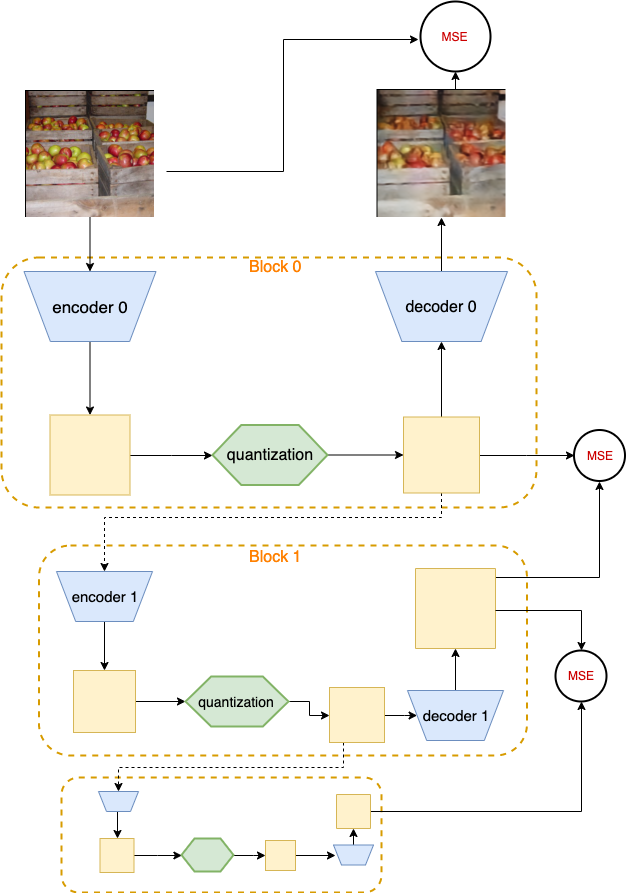
\includegraphics[width=0.45\textwidth]{figs/sqm_cartoon.png}
    \caption{Stacked Quantization Modules. Each level uses its own loss and maintains its own replay buffer. Dotted lines indicate gradient is stopped in the backprop}
    \label{fig:soft_modules}
\end{wrapfigure}

\subsection{Problem Setting}
We consider the problem setting where a stream of samples $x \sim D_t$ arrives from different distributions $D_t$ changing over time $t=1..T$. We have a fixed storage capacity of $C$ bytes where we would like to store the most representative information from all data distributions $D_1,...D_T$. There is notably a trade-off in quality of information versus samples stored. We propose to use a learned compression model, and most crucially, this  model must also be stored within the $C$ bytes, to encode and decode the data samples. 
Another critical requirement is that at anytime $t$ the content of the storage (data and/or compression model) be usable for downstream applications.
%, for example another learner performing online continual classification may operate off this storage. In another setting a learner may obtain access to the storage at a specific $t$ and use it for offline learning.
A key challenge is that the learned compression module will change over time, while we still need to be able to decode the memories in storage. 

The high level training of the online learned compression is described in Alg.~\ref{algo:vqr}. Random memories are decoded and used to train the current compression module, at the same time this also allows us to re-encode those memories using the update weights.  The approach also incorporates a form of replay to address drift and reduce forgetting.  In the rest of this section we discuss the architecture, objective and storage we propose. 




\subsection{Vector Quantized VAE}
Variational Autoencoders (VAE) \citep{kingma2013auto} consist of two parts: the encoder network parameterizes the posterior distribution $q(z|x)$ and the decoder network $p(x|z)$ aims to reconstruct the original input $x$ from the inferred latent variables $z$. In a standard VAE the prior and posterior distributions are usually Gaussian with diagonal covariance. On the other hand Vector Quantized Autoencoders (VQ-VAE) use a discrete latent representation instead \citep{van2017neural}. This model additionally keeps an embedding table $E \in \mathbb{R}^{K \times D}$, consisting of $K$ vectors of size $D$. Given an input (e.g. an RGB image), the encoder first encodes it as a $H_h \times W_h \times D$ tensor, where $H_h$ and $W_h$ denote the height and width of the latent representation. Then, every $D$ dimensional vector goes through a discretization bottleneck using a nearest-neighbor lookup on the embedding table. Specifically,  $z_{ij} = \argmin_{e \in E} || \texttt{enc}(x)_{ij} - e ||_2$. 
%\vspace{-0.1cm}
%\begin{equation*}
 %   z_{ij} = \argmin_{e \in E} || \texttt{enc}(x)_{ij} - e ||_2
%\end{equation*} 
%\vspace{-0.05cm}
The output of the discretization step is then fed through the decoder. The gradient of this  non-differentiable step is approximated using the straight-through estimator. A key property to notice is that to reconstruct the input, only the $H_h \times W_h$ indices are required, thus yielding very powerful compression \citep{van2017neural}. The full VQ-VAE objective, $L_{vq}$ is given in \citet{van2017neural}.



\subsection{Stacked Quantization Modules}
To ensure adaptivity of the compression model, we adopt a Stacked Quantization Modules (SQM). Each module contains a VQ-AE and a corresponding index buffer of adaptive capacity. Its input is the $z_q^{(i-1)}$ from the previous layer. A full diagram of the Stacked Quantization Modules (SQM) is given in Figure~\ref{fig:soft_modules}. Each module reconstructs its input from latent representation $z_q^{i}$, where $\textsc{BITS}(z_q^{i}) < \textsc{BITS}(z_q^{(i-1)})$. The compression rate at a given block is given by
$$
    \frac{H \times W \times C \times  \log_2{(256)}}
         {N_c \times H_h_i \times W_h_i \times \log_2{(K_i)}}
$$
Thus the compression rate is controlled by: $K_i$, the number of embeddings in the codebooks of block $i$, the spatial dimension of the latent rep ($H_{hi}$, $W_{hi}$) and the number of codebooks $N_c_i$ 



VQVAE-2 \citep{razavi2019generating} also uses a multi-scale hierarchical organization, where unlike our SQM the top level models global information such as shape, while the bottom level, conditioned on the top one, models local information. While this architecture is tailored for generative modeling, it is less attractive for compression, as both the bottom and top quantized representations must be stored for high quality reconstructions.

Notably unlike VQVAE-2 \citep{razavi2019generating}, each module is learned greedily without backward communication between modules using the current estimate of $z_q^{(i-1)}$ similar to \cite{belilovsky2019decoupled,nokland2019training}. This formulation is important for allowing the modules to each converge as quickly as possible at their respective resolution. In other words a subsequent block is not required to build representations which account for all levels of compression, thus minimizing interference across resolutions. This rapid convergence is particularly important for the case of online continual learning. 

\subsection{Multi-Level Storage}\label{sec:adap}
Our aim is to store the maximum number of samples in the allotted $C$ bytes of storage, while assuring their quality, and our ability to reconstruct them. The SQM allows us to implement a Multi-Level storage, wherein each module stores samples at its respective scale. Samples are stored at different levels based on the compressors' current ability to compress them. When replay occurs, a sample may be able to propogate into a lower level (and thus permit more samples to enter the storage). This process is summarized in Alg~\ref{algo:adapcomp}. \mynotesLC{In practice, both the SQM training and the sample recompression are done in a single forward pass, allowing for fast training.}

 Such an approach is particularly helpful in the online continual learning setting and allows knowledge retention before the compressor network has learned a valid representations. Note that as per Alg~\ref{algo:adapcomp}, samples can be completely uncompressed until the first module is able to effectively encode them.  This can be crucial in some cases, if the compressor has not yet converged, to avoid storing poorly compressed representations.  Further taking into account that compression difficulty is not the same for all datapoints, this allows use of more capacity for harder data, and fewer for data.

 We also note, since we maintain stored samples at each module and the modules are decoupled, that such an approach allows to distribute training the individual modules in parallel and in an asynchronous manner \citep{belilovsky2019decoupled}.


\subsection{Multi-Level Reservoir Sampling}
Reservoir Sampling (RS) is a critical component of selecting a representative set of samples in continual classification~\cite{chaudhry2019continual}. Its popularity is due to two reasons. First, it gives in expectation a sample representative of the whole data stream.  Second, it is a conceptually simple algorithm, easy to implement, and gives strong empirical results. Indeed more sophisticated approaches can often be outperformed by basic RS in \cite{chaudhry2019continual}.

With this motivation, we need to adapt RS to a multi-level storage settings. There a few challenges. First, in our model the capacity in terms of samples is not fixed. RS adds a new point with prob. $p=\frac{\text{buffer capacity}}{\text{points seen so far}}$. However in practice, the buffer capacity actually \emph{increases} as the compressor network gets better. We therefore estimate it using the current capacity at the time of buffer addition. In the same vein, one could argue that in practice the compressor network's sample capacity is actually bigger than the amount of samples it is currently storing since old samples were added when the buffer was less performant. However, since the points get re-compressed during rehearsal, this issue is mostly resolved.

Sample selection for deletion and sampling is also more complex than in standard RS. While it would be more advantageous to remove datapoints from the least compressed representation level, doing so introduces a bias; some classes may be harder to compress, and removing them more frequently would result in more forgetting of said class. To address this issue, we perform all buffer deletion (and insertion) agnostic to the level of the sample. When memory must be freed, samples are deleted from every block such that their relative memory consumption does not change.
    

%           ALGORITHMS 
% ---------------------------------------------------------





%          End of Algorithms Section 
% ------------------------------------------------------



%\subsection{Using Index Collapse to our advantage}
%\begin{itemize}
 %   \item Start with a high number of embeddings. 
  %  \item When replaying, reorder and compress the codebook! Underuse of embeddings is not a bad thing for compression --> less bits per items
%\end{itemize}


%           BUFFER INDEX UPDATE
% ---------------------------------------------------------
\begin{minipage}{\textwidth}
\begin{minipage}{0.45\textwidth}
\begin{algorithm2e}[H]\small
\SetAlgoLined
  \DontPrintSemicolon
    \KwIn{Memory $\mathcal{M}$, Autoencoder $AE$ with $L$ levels, data $D$, distortion threshold $d_{th}$}
    
\For{$x \in D$}{
    $hid_x$, $block_{id}$ = \textst{AdapCompress}($x$, $AE$, $d_{th}$) \\
    
    \,\,\,\texttt{\% Delete Old Repr.} \\
    \textst{DELETE}($\mathcal{M}$[$x$]) \\
    \,\,\,\texttt{\% Add new one} \\
    \textst{ADD}($\mathcal{M}$, $hid_x$) 
}

 \caption{Update Buffer Represent.}
\label{algo:vqr}
    
   % \end{edit}
\end{algorithm2e}
\end{minipage}
\qquad
%           RESERVOIR ADD 
% ------------------------------------------------------
\begin{minipage}{0.5\textwidth}
\begin{algorithm2e}[H]\small
\SetAlgoLined
  \DontPrintSemicolon
    \KwIn{Memory $\mathcal{M}$ with capacity $C$ (bytes), sample $x$}
    
    %\,\,\,\texttt{\% Number of uncompressed samples buffer can store} \\
    $N_{reg}$ = $\frac{C}{\textst{BYTES}(x)}$
    
    %\,\,\,\texttt{\% Calculate probability of adding x} \\
    
    capacity = $\max$(\ $N_{reg}$, \textst{NUM SAMPLES }($\mathcal{M}$)\ ) 
    
    %\,\,\,\texttt{\% Probability of adding x} \\
     \,\,\,\texttt{\% Calculate probability of adding x} \\
    add $\sim \mathcal{B}(\frac{\text{capacity}}{\text{SAMPLE AMT SEEN SO FAR}})$
    
    \,\,
    \If{add}
    {
        $hid_x$, $block_{id}$ = \textst{AdaptCompress}($x$, $AE$, $d_{th}$) \\
       % empty space =  \text{BYTES}($hid_x$) - \textst{FREE SPACE}($\mathcal{M}$)
      %  \,\,\,\texttt{\% Note: implementation is much faster but same idea} \\
        \While {\text{BYTES}($hid_x$) - \textst{FREE SPACE}($\mathcal{M}$) $> 0$}{
            \textst{DELETE RANDOM}($\mathcal{M}$) \\
         %   empty space \gets  \text{BYTES}($hid_x$) - \textst{FREE SPACE}($\mathcal{M}$)
        }
        
    }
    

 
 \caption{Add to Memory}
\label{algo:vqr}
   % \end{edit}
\end{algorithm2e}
\end{minipage}
\end{minipage}
% ---------------------------------------------------------
%                      Experiments
% ---------------------------------------------------------
\section{Experiments}

We evaluate the efficacy of the proposed methods on a suite of canonical and new experiments. In  Section \ref{sec:can_cl} we present results on standard supervised continual learning benchmarks on CIFAR-10. In Section~\ref{sec:off} we evaluate other downstream tasks such as standard iid training applied on the storage at the end of online continual compression. For this evaluation we consider larger images from Imagenet, as well as on LiDAR data.  

\subsection{Online Continual Classification}
\label{sec:can_cl}
Although CL has been studied in generative modeling \citep{ramapuram2017lifelong,lesort2018generative,Zhai2019LifelongGC,lesort2019marginal} and reinforcement learning \citep{kirkpatrick2017overcoming,fernando2017pathnet,riemer2018learning}, supervised learning is still the standard for evaluation of new methods. Thus, we focus on the online continual classification of images for which our approach can provide a complement to experience replay. In this setting, a new task consists of new image classes that the classifier must learn, while not forgetting the previous ones. The model is only allowed one pass through the data \citep{lopez2017gradient,chaudhry2018efficient,aljundi2019online,chaudhry2019continual}. The online compression here takes the role of replay buffer in replay based methods such as \cite{chaudhry2019continual,aljundi2019online}. In short, we apply Algorithm~\ref{algo:vqr}, with an additional online classifier being updated at line 13.

Here we consider the more challenging \textit{shared-head} setting, where the model is not informed of the task (and thereby the subset of classes) at test time. This is in contrast to other (less realistic) CL classification scenarios where the task, and therefore subset of classes, is provided explicitly to the learner \cite{farquhar2018towards}.

%which have albeen studied thus far, a design chose of  importance is the \textit{test-time task label assumption} \citep{farquhar2018towards}. It is much easier for a model to operate if the tasks are specified at test time. This however is less natural as a learner acquiring new knowledge  such as object categories will rarely be guided at test time about which category it is to classify. 
%To ground this in a concrete example, we can think of a robot continually learning to grab new objects. In this setting, a new object represents a new task. If a human (or a oracle) is always helping the robot by informing it of the nature of the next object to grab, then the assumption of the task label at test time isn't a bad idea. In this case, the robot can learn different policies for each objects, which can greatly reduce interference and thus forgetting. However, if we are interested in a more autonomous model, that assumption should be relaxed. Naturally, the continual learning becomes more challenging. Both settings are useful for \textit{real-life} continual learning. Thus, they are both studied in Section \ref{sec:can_cl} under the \textit{shared-headed} (no task label given) and \textit{multi-head} (task label given) nomenclature.
For this set of experiments, we primarily report accuracy, i.e. $\dfrac{1}{T} \sum_{i=1}^T R_{T,i}$, and forgetting, i.e. $\dfrac{1}{T-1} \sum_{i=1}^{T-1} \max(R_{:,i}) - R_{T,i}$
with $R \in \mathbb{R}^{TxT}$ representing the accuracy matrix where $R_{i,j}$ is the test classification accuracy on task $j$ when task $i$ is completed.


\paragraph{Baselines}
A basic baseline for continual supervised learning is Experience Replay (\textbf{ER}). It consists of storing old data in a buffer to replay old memories. Due to its very simple nature, this baseline was often omitted in continual learning papers. However, recent research made it clear that it is a critical baseline to consider, and in some settings is actually state-of-the-art \citep{chaudhry2019continual,aljundi2019online,rolnick2018experience}. SQM can be viewed as an add-on to ER that incorporates online continual compression. In addition we consider the following baselines. \textbf{iid online} (upper-bound)
 trains the model with a single-pass through the data on the same set of samples, but sampled iid. \textbf{iid offline} (upper-bound) evaluates the model using multiple passes through the data, sampled iid. We use 5 epochs in all the experiments for this baseline. \textbf{fine-tuning} trains continuously upon arrival of new tasks without any forgetting avoidance strategy. \textbf{iCarl} \citep{rebuffi2017icarl} incrementally classifies using a nearest neighbor algorithm, and prevents catastrophic forgetting by using an stored samples. \textbf{GEM} \citep{lopez2017gradient} uses stored samples to avoid increasing the loss on previous task through constrained optimization. It has been shown to be a strong baseline in the online setting. It gives similar results to the recent A-GEM \cite{chaudhry2018efficient}. \textbf{ER-MIR} \citep{aljundi2019online} controls the sampling of the replays to bias sampling towards samples that will be forgotten. \mynotesLC{We note that the ER-MIR critera is orthogonal to SQM, and both can be applied jointly. We leave this as future work.}
% \begin{itemize}
%     \item \textbf{iid online} (upper-bound)
%     considers training the model with a single-pass through the data on the same set of samples, but sampled iid.
%     \item \textbf{iid offline} (upper-bound)
%     evaluates the model using multiple passes through the data, sampled iid. We use 5 epochs in all the experiments for this baseline.
%     \item \textbf{fine-tuning} trains continuously upon arrival of new tasks without any forgetting avoidance strategy.
%     \item \textbf{iCarl} \citep{rebuffi2017icarl} incrementally classifies using a nearest neighbor algorithm, and prevents catastrophic forgetting by using an stored samples.
%     \item \textbf{GEM} \citep{lopez2017gradient} uses stored samples to avoid increasing the loss on previous task through constrained optimization. It has been shown to be a strong baseline in the online setting. It gives similar results to the recent A-GEM \cite{chaudhry2018efficient}.
%     \item  \textbf{ER-MIR} \citep{aljundi2019online} controls the sampling of the replays to bias sampling towards samples that will be forgotten.
% \end{itemize}

We evaluate with the standard CIFAR-10 split \citep{aljundi2018Online}, where 5 tasks are presented sequentially, each adding two new classes. Evaluations are shown in Table~\ref{tab:cifar10_er_main}. 
%Here SQM refers to our model without the multi-level storage (all memories are stored at the final compression level). A-SQM refers to the full model with adaptive compression, which performs better.
Due to our improved storage of previous data, we observe significant improvements over the other methods and baselines at various memory sizes. This is despite the drifting representation and decoder model. We can contrast SQM's performance with ER's to understand the net impact of our compression scheme. Specifically, SQM improves over ER by 12.4\% and 13.1\% in the M=20 and M=50 case, highlighting the effectiveness of online compression. Our approach only lags ER-MIR in forgetting in the M=50 setting. However, this method is orthogonal to ours and could thus be used jointly.

We also implemented the baseline of \cite{riemer2018learning} that uses a discrete autoencoder with gumbel softmax \citep{jang2016categorical}. \mynotesLC{We benchmarked our implementation on the Incremental CIFAR-100 multi-head experiment \cite{lopez2017gradient}. By using our (more sophisticated) architecture, we were able to get \textbf{60.3} vs the reported \textbf{43.7} using a buffer of size 200. While SQM performs similarly in this setting \textbf{(65.1)}, its compressed representations incur significantly less drift compared to \cite{riemer2018learning}. In the single head setting, this distortion becomes much more problematic as the classifier learns to assign old labels to blurry images, leading to poor performance. We show an example of this drift in Fig. \ref{fig:dist_comparison}.}


%Unfortunately we were not able to get this model to learn online to any reasonable degree. Indeed we emphasize that an off-the-shelf learned compression approach applied naively is unlikely to yield meaningful samples in online training. 
%Our use of the fast converging Multi-level VQ-VAE and rehearsal are essential to permit the final memories to be plentiful and usable. 

The CIFAR-10 dataset has a low resolution ($3 \times 32 \times 32$) and uses a lot of data per task (10K samples). These two characteristics might leave the online compression problem easier than in a real-life scenario. Specifically, if the first tasks are long enough and the compression rate is not too large, the model can quickly converge and thus not incur too much representation drift. \mynotesLC{Indeed, we found that using a single module worked best for this task, as adding more modules was not worth the additional storage cost}. For these reasons, we study the adaptive instantiation of our proposed method (A-SQM) in more challenging settings presented in the next section. 

\begin{figure}[h!]
    \centering
    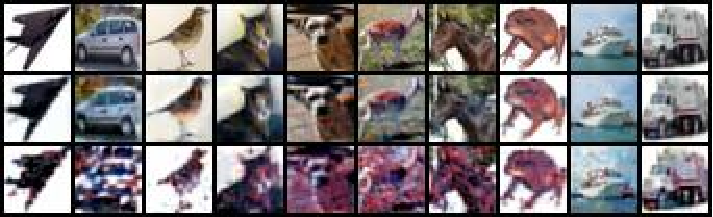
\includegraphics[width=0.5\textwidth]{figs/recon_comp.pdf}
    \caption{\mynotesLC{Bottom row: random buffer reconstructions using \cite{riemer2018learning}. Middle row: random buffer reconstructions using SQM. Top row: corresponding original image. Columns are ordered w.r.t their entry time in the buffer, from oldest to newest. All samples above were obtained from the disjoint CIFAR-10 task, and are 12$\times$ smaller than their original image.}}
    \label{fig:dist_comparison}
\end{figure}

%In this section, we study the proposed methodology under the standard evaluation protocol for CL: incremental image classification. The more challenging datasets which as been studied thus far are CIFAR (cite) and Mini-ImageNet. The former was initially studied \todo{cite} in the multi-head scenario under the 100 class version of the dataset, i.e. CIFAR-100. This experiment consists of 20 consecutive tasks, each adding five new classes. More recently, it was studied in the shared-head scenario under its 10 class version, CIFAR-10. This experiment consists of 5 tasks, each adding two new classes. 
%In this work, we study both settings, keeping the numbers of classes and tasks identical to the literature just mentioned. Next, Mini-ImageNet was studied in \todo{cite}. It is of much higher resolution than CIFAR as well as more challenging. The current state of the supervised CL technology doesn't permit much learning in the shared-head scenario. 
%Thus, only the multi-head setting will be studied for the Mini-ImageNet dataset. The scenario is identical to the CIFAR-100 experiment w.r.t number of tasks and of classes. 

%\mynotesLC{\textbf{result analysis} We see that for }

%\todo[color=red]{insert preliminary results for continual supervised learning}
%\todo[color=orange]{Describe continual supervised learning results}
%\todo[color=yellow]{insert final results for continual supervised learning}


% %%%% CIFAR-10
\begin{table}
    \centering
    \resizebox{\textwidth}{!}{%
    \begin{tabular}{ll}
    \begin{tabular}{c c c}
&\multicolumn{2}{c}{Accuracy ($\uparrow$)} \\\hline
                 & $M=20$ & $M=50$  \\\hline \hline
    iid online     &$60.8\pm1.0$ &$60.8\pm1.0$\\
    iid offline     &$79.2\pm 0.4$ &$79.2\pm 0.4$\\\noalign{\hrule height 1pt}
    GEM   \citep{lopez2017gradient}   &$16.8 \pm 1.1$& $17.1 \pm 1.0$\\
    iCarl (5 iter)  \citep{rebuffi2017icarl}   &$28.6 \pm 1.2$ & $33.7 \pm 1.6$ \\
    fine-tuning &$18.4\pm0.3$& $18.4\pm0.3$\\
     ER&$27.5\pm 1.2$ &$33.1\pm 1.7$\\
    ER-MIR \citep{aljundi2019online}& $29.8\pm1.1$ &$40.0 \pm 1.1$ \\
   % SQM (ours) & $\bm{40.2 \pm 1.2}$ & $\bm{45.7 \pm 0.8}$\\ %ca cest pas adaptive
   \citep{riemer2018learning} & $25.5\pm2.0$ &$28.8 \pm 2.9$ \\
    SQM (ours) & $\bm{39.9 \pm 0.8}$ & $\bm{46.2 \pm 0.8}$ \\ %this is the adaptive one
    % \multicolumn{4}{c}{}\\
\end{tabular}
&
\begin{tabular}{c c}
\multicolumn{2}{c}{Forgetting ($\downarrow$)} \\\hline
     $M=20$ & $M=50$  \\\hline \hline
    N/A &N/A\\
  N/A&N/A\\\noalign{\hrule height 1pt}
        $73.5 \pm 1.7$ & $70.7 \pm 4.5$ \\
    $49 \pm2.4$& $40.6\pm1.1$\\
  $85.4 \pm 0.7$  & $85.4 \pm 0.7$\\
    $50.5\pm 2.4$&$35.4\pm 2.0$ \\
    $50.2\pm 2.0$&$\bm{30.2 \pm 2.3}$ \\
    $71.5\pm 2.8$&$ 67.2 \pm 3.9$ \\
   % $49.2 \pm 1.8$ & $43.9 \pm 1.4$ \\
    $50.5 \pm 1.1 $ & $42.8 \pm 1.3$ \\
      %  \multicolumn{4}{c}{}\\
\end{tabular}
\end{tabular}
}
\caption{Shared head results on disjoint CIFAR-10. Total memory per class $M$ measured in sample memory size. We report  (a) Accuracy, (b) Forgetting (lower is better). }
\label{tab:cifar10_er_main}
\end{table}

\subsection{Offline Evaluation on Larger Images and LiDAR}
\label{sec:off}
Besides the standard continual classification setup, we propose several other evaluations that attempt to determine the effectiveness of the stored data and compression module after learning online compression. %learning compression online compression.

\paragraph{Offline training on Imagenet} We compare the effectiveness of the stored memories of SQM after a certain amount of online continual compression. We do this by training in a standard iid way an offline classification model using only reconstructions obtained from the storage sampled after online continual compression has progressed for a period of time.  In each case we would have the same sized storage available. We remind the reader that simply having more stored memories does not amount to better performance as their quality may be severely degraded and affected by drift. 

We use the mini-imagenet dataset, but resized to $128 \times 128$, larger than the typical size used as we aim to emphasize the utility of this methods for larger inputs. Online continual compression arrives using the standard split-minimagenet from \cite{chaudhry2019continual}, which yields 20 different tasks and 100 classes total. After all samples have been seen and stored as best as possible in storage size $C$ by Algorithm~\ref{algo:vqr}, we train a Resnet18 model (similar to the one used in \cite{chaudhry2019continual} adjusted for larger input size) using the stored samples. We train with SGD and a learning rate of 0.1, with early stopping using a validation set. The storage size $C$ is equivalent to 1000 uncompressed samples. Results of this evaluation are shown in Table ~\ref{tab:offline}. 


Using this evaluation we first compare a standard reservoir sampling approach on uncompressed data to a 2 module A-SQM using the same size storage. We observe that performance is drastically increased using the compressed samples. We then use this to perform a series of ablations to demonstrate each component of our proposal is important. First we ablate the modular training, meaning the model is trained end-to-end instead of greedily, which is unable to perform well online. Secondly we consider not using the adaptive compression scheme described in Sec~\ref{sec:adap}, thus all samples are compressed at the bottom level. This greatly decreases performance, likely due to very low sample quality that cant be recovered. We then consider removing the 2nd Module showing that multiple levels aid in performance. We additionally illustrate the change in the amount of samples stored at each level by adaptive storage in Figure~\ref{fig:adaptive}

%\mynotesEB{Add something}
%Our use of the fast converging Multi-level VQ-VAE and rehearsal are essential to permit the final memories to be plentiful and usable.

\begin{table}
    \centering
    \begin{tabular}{c|c}
&Accuracy \\\hline
    RS &$5.2$\\
    \textbf{2 Module A-SQM (ours)} & $\textbf{19.8}$ \\\hline
    Ablate Modular Training & $12.7$ \\
    Ablate Adaptive Compression  & $10.8$ \\ % \hline
    Ablate 2nd Module & $9.61$ \\
    Ablate 2nd Module \& Adaptive compression & $12.0$  \\ \hline

\end{tabular}
\caption{Offline training evaluation of storage from online continual compression. We see a clear gain over a standard Reservoir sampling approach. We then ablate each component of our proposal showing each component is important. Note storage used in each experiment is identical (including accounting for model sizes).}\label{tab:offline}
\end{table}


\begin{figure}
    \centering
    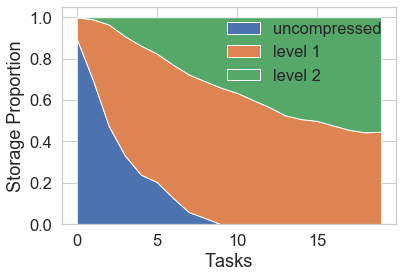
\includegraphics[width=0.4\textwidth]{figs/adaptative_buffer_prop.png}
    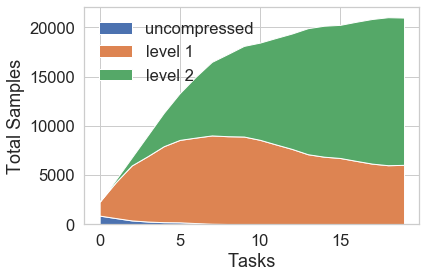
\includegraphics[width=0.4\textwidth]{figs/adaptative_buffer_tot_samples.png}
    \caption{Evolution of the storage proportion (left) and total number of stored samples (right) for different compression levels in A-SQM. Throughout, our method reduces the proportion of lower level resolutions, allowing an increasing total amount of stored samples.}
    \label{fig:adaptive}
\end{figure}



\paragraph{LiDAR} Range data can be very large and storage inefficient, it is also often collected by vehicles in potentially changing environments. Efficient storage can be important for having more representative data in downstream applications. Here we show qualitatively several examples of applying this.   
For this experiment we use the Kitti Dataset \citep{geiger2013vision}, which contains 61 LiDAR scan recordings, each belonging to either the ``residential", ``road", ``city" environments. We use a 2 module SQM and perform online continual compression. The online compression is presented one by one with scans from each environment, we present all the recordings from one environment, before moving on to another. 

The data is processed as in \cite{caccia2018deep}, where points from the same elevation angle are sorted in increasing order of azimuth angle along the same row. This yield a 2D grid, making it compatible with the same architecture used in the previous experiments. We show qualitative results in Figure~\ref{fig:lidar_qualitative}, using a 3 Block SQM, observe that we are able to effectively reconstruct the LiDAR samples. We note that reconstruction quality has been previously linked to performance on downstream tasks such as SLAM \cite{zhang2014loam}

%\begin{figure}
%    \centering
%    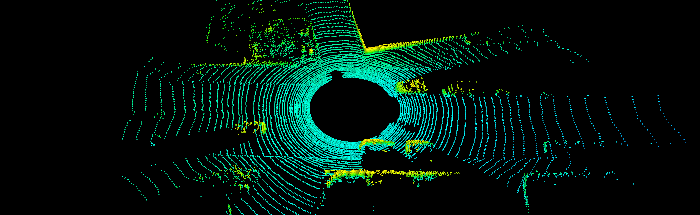
\includegraphics[width=7cm]{figs/lidar_og.png}
%    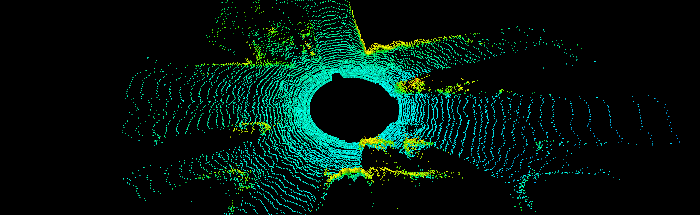
\includegraphics[width=7cm]{figs/lidar_c1.png}
%    \caption{\textbf{Top:} original LiDAR image. \textbf{Bottom:} reconstructed LiDAR image compressed $6.5 \times$. We observe that the main structures are largely unaffected.}
%    \label{fig:lidar_qualitative}
%\end{figure}

\begin{figure}%[!h]
        \centering
        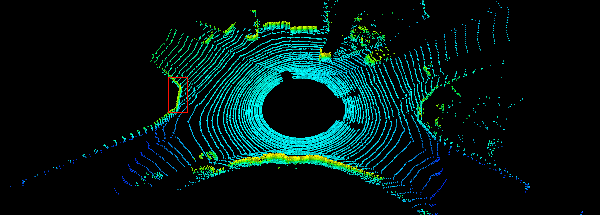
\includegraphics[width=.4\textwidth]{figs/good_og_s.png} \ \ \ %\vskip 1mm
        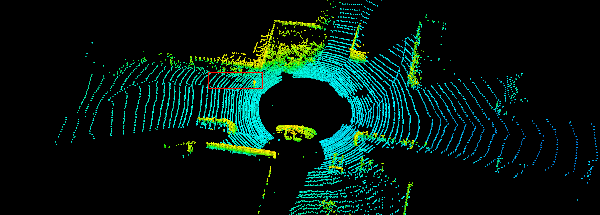
\includegraphics[width=.4\textwidth]{figs/flawed_og_s.png} \vskip 2mm
        
        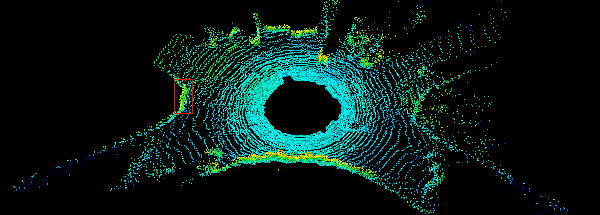
\includegraphics[width=.4\textwidth]{figs/good_8_s.png} \ \ \ %\vskip 1mm
        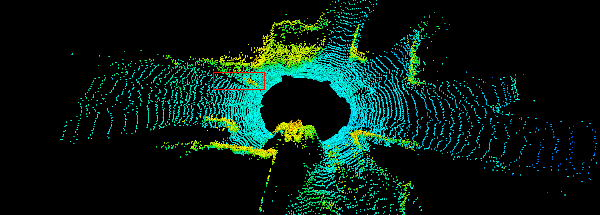
\includegraphics[width=.4\textwidth]{figs/flawed_8_s.png} \vskip .5mm
        
        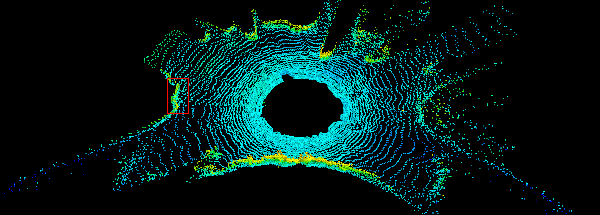
\includegraphics[width=.4\textwidth]{figs/good_16_s.png}\ \ \ \ %\vskip 1mm
        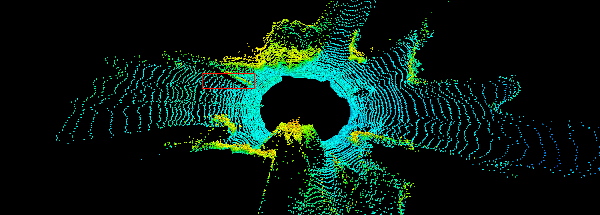
\includegraphics[width=.4\textwidth]{figs/flawed_16_s.png} \vskip .5mm
        
        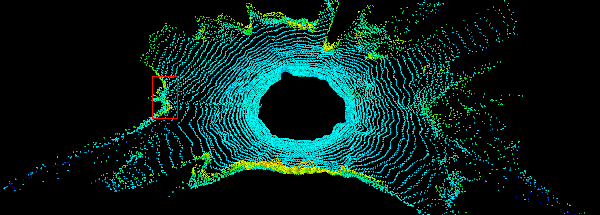
\includegraphics[width=.4\textwidth]{figs/good_32_s.png} \ \ \  
        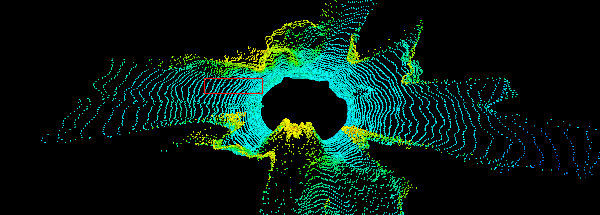
\includegraphics[width=.4\textwidth]{figs/flawed_32_s.png}  \vskip .5mm

\caption{\mynotesLC{Top row are real uncompressed test set lidar scans. Rows two, three and four are reconstructions with compression rate 8, 16, and 32$\times$. Regions of interest are highlighted in red. In the left column, we note that all compression levels retain the essential information, albeit some far way obstacles are slightly deformed. In the right column, a thin obstacle is present in the first two levels, but is absent in the third level.}}
\label{fig:lidar_qualitative}
\end{figure}


% % @Eugene: dont hate me, ill figre it out later
% %\begin{wrapfigure}[20]{L}{0.50\textwidth}
% \begin{figure}
%     \centering
%     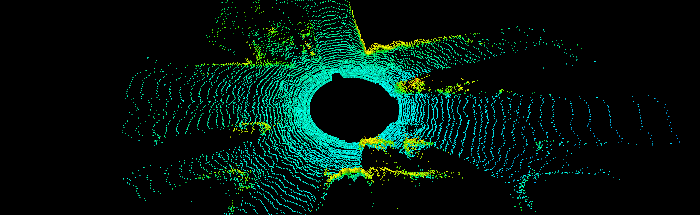
\includegraphics[width=0.4\textwidth]{figs/lidar_c1.png}
%     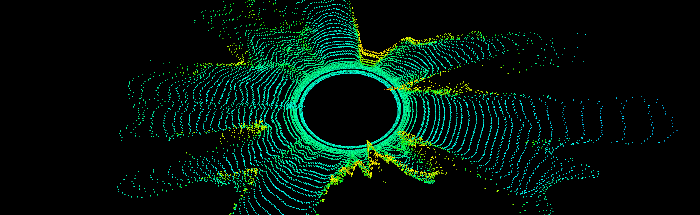
\includegraphics[width=0.4\textwidth]{figs/lidar_c2.png}
%     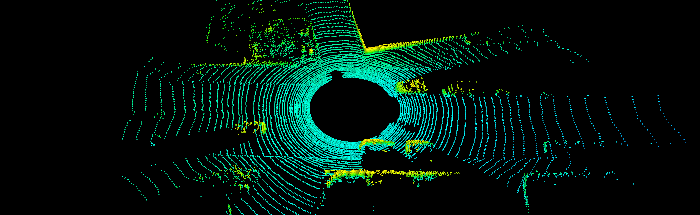
\includegraphics[width=0.4\textwidth]{figs/lidar_og.png}
%     \caption{(a) Compressed LiDAR image (b) original (c) Reference real image}
%     \label{fig:lidar_qualitative}
% \end{figure}
% %\end{wrapfigure}


% ---------------------------------------------------------
%                      Conclusion
% ---------------------------------------------------------
\section{Conclusion}
We have introduced online continual compression. We have shown how replay combined with a novel Multi-level quantization module can allow for the compression model to be learned online and yield a large decodable dataset despite representation and model drift. We have shown effectiveness of this online compression approach on standard continual classification benchmarks, as well as for compressing larger images and LiDAR data. We believe future work can consider dealing with temporal correlations for video and reinforcement learning tasks, as well as improved prioritization of samples for storage.  


%\clearpage
% ---------------------------------------------------------
%                      TODOs / Misc
% ---------------------------------------------------------
%\section{Remaining stuff}

%\begin{enumerate}
 %   \item Would be nice to have a fully mapping task for LiDAR. Say you deploy a robot in an unknown environment, and you want it to collect data. Given a fixed memory, compression becomes really important!

  %  \item Classification Task for LiDAR ? SLAM, or 3D object detection from point clouds 
%    I would like said task to be super close to real life
   % \begin{enumerate}
 %       \item Data comes in temporally corelated $\rightarrow$ Can ER solve this ?
  %      \item Semi-Supervised setting: only a few frames have labelled objects. This would make the importance of large buffer more important, as it takes a lot of data to properly decorellate frames (TODO)
                
   % \end{enumerate}
    
        
    %\item Link with MIR: How much does codebook overlap predict forgettability ?
    
    %\item Can we show than when a DGM doing compression (vs DDM) has learned a concept, less rehearsal is needed ? Would motivate latent rehearsal

%\end{enumerate}
%\subsubsection*{Author Contributions}
%If you'd like to, you may include  a section for author contributions as is done
%in many journals. This is optional and at the discretion of the authors.

%\subsubsection*{Acknowledgments}
%EB acknowledges funding from IVADO






%%%% CIFAR-10
% \begin{table}
%     \centering
%     \resizebox{\textwidth}{!}{%
%     \begin{tabular}{ll}
%     \begin{tabular}{c c c}
% &\multicolumn{2}{c}{Accuracy} \\\hline
%                  & $M=25$ & $M=50$  \\\hline \hline
%     ER&$26.1 \pm 0.4$ &$31.2 \pm 0.4$\\
%     SQM (ours) & $40.5 += 0.7$ & $\bm{45.9 \pm 1.1}$\\
%     A-SQM (ours) & $\bm{42.4 += 0.9}$ & $\bm{46.2 \pm 0.6}$ \\
%     % \multicolumn{4}{c}{}\\
% \end{tabular}
% &
% \begin{tabular}{c c}
% \multicolumn{2}{c}{Forgetting} \\\hline
%      $M=25$ & $M=50$  \\\hline \hline
%     $59.4 \pm .50 $&$53.0 \pm 0.7$ \\
%     $40.7 \pm 0.9$ & $36.5 \pm 1.2$ \\
%     $39.3 \pm 1.1$& $36.1 \pm 0.6$ \\
%       %  \multicolumn{4}{c}{}\\
% \end{tabular}
% \end{tabular}
% }
% \caption{Shared head results on disjoint CIFAR-10. Total memory per class $M$ measured in sample memory size. We report  (a) Accuracy, (b) Forgetting (lower is better). }
% \label{tab:cifar10_er_main}
% \end{table}



%\subsection{On convergence speed}
%\begin{itemize}
 %   \item Can we justify the convergence speed by looking at the variance in the gradient ?
  %  \item Can we show that deeper modules need more rehearsing ? We could look at the speed of drift in the reconstructions. 
%\end{itemize}

%\subsection{Reusing Encoder modules}
%\begin{itemize}
 %   \item In Image classification for RGB data. See \url{https://arxiv.org/pdf/1803.06131.pdf}
  %  \item 
%\end{itemize}

%\subsection{Is ER enough to properly decorrelate temporally adjacents frames ?}

% ---------------------------------------------------------
%                      Ablation Study
% ---------------------------------------------------------

%\todo[color=orange]{add preliminary results of quality/diversity space ablation}

%\section{Ablation Study}
%\begin{itemize}
%    \item Show that modular training does not hurt final performance (i.e. same compression ratio with only 1 quantization). This will entail that you get compressed intermediate representations for free. 
%    \item Show that modular training converges faster! If you train the same fixed architecture altogether, look at the time it takes for the first block to reach some fixed error rate. 
%    \item Full Architecture from the start vs Progressive Training. Does it hurt performance ? To be checked
%\end{itemize}


\bibliography{ref}
\bibliographystyle{iclr2020_conference}

%\appendix
%\section{Appendix}
%You may include other additional sections here. 

\end{document}
